% This is "sig-alternate.tex" V2.1 April 2013
% This file should be compiled with V2.5 of "sig-alternate.cls" May 2012
%
% This example file demonstrates the use of the 'sig-alternate.cls'
% V2.5 LaTeX2e document class file. It is for those submitting
% articles to ACM Conference Proceedings WHO DO NOT WISH TO
% Strictly ADHERE TO THE SIGS (PUBS-BOARD-ENDORSED) STYLE.
% The 'sig-alternate.cls' file will produce a similar-looking,
% albeit, 'tighter' paper resulting in, invariably, fewer pages.
%
% ----------------------------------------------------------------------------------------------------------------
% This .tex file (and associated .cls V2.5) produces:
%       1) The Permission Statement
%       2) The Conference (location) Info information
%       3) The Copyright Line with ACM data
%       4) NO page numbers
%
% as against the acm_proc_article-sp.cls file which
% does NOT produce 1) thru' 3) above.
%
% Using 'sig-alternate.cls' you have control, however, from within
% the source .tex file, over both the CopyrightYear
% (defaulted to 200X) and the ACM Copyright Data
% (defaulted to X-XXXXX-XX-X/XX/XX).
% e.g.
% \CopyrightYear{2007} will cause 2007 to appear in the copyright line.
% \crdata{0-12345-67-8/90/12} will cause 0-12345-67-8/90/12 to appear in the copyright line.
%
% ---------------------------------------------------------------------------------------------------------------
% This .tex source is an example which *does* use
% the .bib file (from which the .bbl file % is produced).
% TODO REMEMBER HOWEVER: After having produced the .bbl file,
% and prior to final submission, you *NEED* to 'insert'
% your .bbl file into your source .tex file so as to provide
% one 'self-contained' source file.
% ================= IF YOU HAVE QUESTIONS =======================
% Questions regarding the SIGS styles, SIGS policies and
% procedures, Conferences etc. should be sent to
% Adrienne Griscti (griscti@acm.org)
%
% Technical questions _only_ to
% Gerald Murray (murray@hq.acm.org)
% ===============================================================
%
% For tracking purposes - this is V2.0 - May 2012

\documentclass{sig-alternate-05-2015}
  \pdfpagewidth=8.5truein
  \pdfpageheight=11truein
  
  
% Custom package imports
\usepackage[utf8]{inputenc}
\usepackage{microtype}
\usepackage{booktabs}

\usepackage{graphicx}
\usepackage[utf8]{inputenc}
\usepackage{listings}
\usepackage{cleveref}
\usepackage{textcomp}
\usepackage[usenames, dvipsnames]{color}
\usepackage{url}

% Custom config
\graphicspath{{figures/}}

\definecolor{myviolett}{RGB}{127, 0, 85}
\definecolor{darkred}{RGB}{136, 0, 0}
\definecolor{darkblue}{RGB}{52, 89, 127}
\definecolor{lightgreen}{RGB}{44, 55, 0}

\lstset{
	basicstyle=\ttfamily\scriptsize,
	keywordstyle=\color{darkred}\ttfamily,
	stringstyle=\color{darkblue}\ttfamily,
	commentstyle=\color{lightgreen}\ttfamily,
	breaklines=true,
	aboveskip=.75\baselineskip,
	belowskip=1.5\baselineskip,
	upquote=true,
	showstringspaces=false
}

\lstdefinelanguage{dsl} % Farblich orientiert an Eclipse
{
	morekeywords={
		Feature,
		As,a,
		I, want, to,
		In, order, to,
		Scenario,
		Given, I, am, on, the, screen, 
		when, I, in, the, textfield, type, and,click,button,
		then, the, alert, is,
		Mapping, url,fragment,locator, label, nls, en, driver
	},
	sensitive=false, % keywords are not case-sensitive
	%morecomment=[l]{//}, % l is for line comment
	%morecomment=[s]{/*}{*/}, % s is for start and end delimiter
	morestring=[b]", % defines that strings are enclosed in double quotes
}

\lstdefinelanguage{xtext} % Farblich orientiert an Xtext Doku
{
	morekeywords={
		ID,	STRING, DOUBLE, MESSAGE,
		returns, current
	},
	sensitive=true, % keywords are case-sensitive
	%morecomment=[l]{//}, % l is for line comment
	%morecomment=[s]{/*}{*/}, % s is for start and end delimiter
	morestring=[b]', % defines that strings are enclosed in double quotes
	keywordstyle=\color{myviolett}\ttfamily,
	morekeywords={[2]{Person, UsualCase, Unknown, 
			ResultDeclaration, Query, 
			PlusOrMinus, MetricExpression, MulOrDiv, MetricAtomic, SumFunction, ColumnSelection, MetricsCountFunction, MetricsRef, DoubleConstant,
			RuleBody, RuleSpecification, WarnIf,
			Column, Requirement,
			Operator, RuleAtomic,
			Factor, MetricDefinition, Term,CountFunction, LengthFunction}},
	keywordstyle={[2]{\color{darkblue}}},
	stringstyle=\color{lightgreen}\ttfamily,
}

\crefname{lstlisting}{Listing}{Listings}
\crefname{figure}{Figure}{Figures}

\begin{document}

% Copyright
\setcopyright{acmcopyright}
%\setcopyright{acmlicensed}
%\setcopyright{rightsretained}
%\setcopyright{usgov}
%\setcopyright{usgovmixed}
%\setcopyright{cagov}
%\setcopyright{cagovmixed}


% the DOI
\doi{http://dx.doi.org/xx.xxxx/xxxxxxx.xxxxxxx}

% the ISBN
\isbn{978-1-4503-4486-9/17/04}

\acmPrice{\$15.00}

%
% --- Author Metadata here ---
\conferenceinfo{SAC'17,}{ April 3-7, 2017, Marrakesh, Morocco}
\CopyrightYear{2017} % Allows default copyright year (20XX) to be over-ridden - IF NEED BE.
%\crdata{0-12345-67-8/90/01}
% --- End of Author Metadata ---

\title{A Model-Driven Approach for Behavior-Driven UI Testing
%Possible alternative titles:
%A model driven approach for specifying automated UI tests
%A domain-specific language for defining automated UI tests
%Generating automated UI tests from formal requirement specifications
%Natural-language processing for test generation
%Automating UI tests from a scenario DSL
%\titlenote{(Produces the permission block, and copyright information). For use with SIG-ALTERNATE.CLS. Supported by ACM.}
}
%\subtitle{[Extended Abstract]
%\titlenote{A full version of this paper is available as \textit{Author's Guide to Preparing ACM SIG Proceedings Using \LaTeX$2_\epsilon$\ and BibTeX} at \texttt{www.acm.org/eaddress.htm}}}
%
% You need the command \numberofauthors to handle the 'placement
% and alignment' of the authors beneath the title.
%
% For aesthetic reasons, we recommend 'three authors at a time'
% i.e. three 'name/affiliation blocks' be placed beneath the title.
%
% You are NOT restricted in how many 'rows' of
% "name/affiliations" may appear. We just ask that you restrict
% the number of 'columns' to three.
%
% Because of the available 'opening page real-estate'
% we ask you to refrain from putting more than six authors
% (two rows with three columns) beneath the article title.
% More than six makes the first-page appear very cluttered indeed.
%
% Use the \alignauthor commands to handle the names
% and affiliations for an 'aesthetic maximum' of six authors.
% Add names, affiliations, addresses for
% the seventh etc. author(s) as the argument for the
% \additionalauthors command.
% These 'additional authors' will be output/set for you
% without further effort on your part as the last section in
% the body of your article BEFORE References or any Appendices.

\numberofauthors{1} %  in this sample file, there are a *total*
% of EIGHT authors. SIX appear on the 'first-page' (for formatting
% reasons) and the remaining two appear in the \additionalauthors section.
%
\author{
% You can go ahead and credit any number of authors here,
% e.g. one 'row of three' or two rows (consisting of one row of three
% and a second row of one, two or three).
%
% The command \alignauthor (no curly braces needed) should
% precede each author name, affiliation/snail-mail address and
% e-mail address. Additionally, tag each line of
% affiliation/address with \affaddr, and tag the
% e-mail address with \email.
%
% 1st. author
\alignauthor
%Christoph Rieger\\
%       \affaddr{ERCIS}\\
%       \affaddr{ERCIS, University of Münster}\\
       % TODO wirklich die Post-Adresse?
   %    \affaddr{Leonardo Campus 3}\\
   %    \affaddr{48149 Münster, Germany}\\
%       \affaddr{Münster, Germany}\\
%       \email{christoph.rieger@ercis.de}
- blinded for review -
}
%TODO weitere Autoren

% There's nothing stopping you putting the seventh, eighth, etc.
% author on the opening page (as the 'third row') but we ask,
% for aesthetic reasons that you place these 'additional authors'
% in the \additional authors block, viz.
%\additionalauthors{Additional authors: John Smith (The Th{\o}rv{\"a}ld Group, email: {\texttt{jsmith@affiliation.org}}) and Julius P.~Kumquat (The Kumquat Consortium, email: {\texttt{jpkumquat@consortium.net}}).}
\date{1 February 2017}
% Just remember to make sure that the TOTAL number of authors
% is the number that will appear on the first page PLUS the
% number that will appear in the \additionalauthors section.

\maketitle
\begin{abstract}
Behavior-driven development (BDD) brings requirement specifications and their test cases closer together by using an ubiquitous language to describe requirements that are automatically mapped to test methods.
Although, industry-proven tools support this automated requirement mapping, the test methods need to be implemented manually.
Further, additional artifacts such as UI descriptions are not formally included in requirement definitions so that they drift apart leading to inconsistencies between the expected design and the described behavior of the application.
The approach presented in this paper includes UI descriptions in format of wireframes into BDD like requirement specifications to enable fully generated and automatically executable test cases.
The wireframes are created with Wireframesketcher a tool that supports designs for multiple UI-styles such as HTML or iOS and is well integrated in the Eclipse IDE.
The requirements descriptions are defined in a domain-specific language (DSL) that abides to the rules of the ubiquitous language enhanced by references to screens and widgets from the Wireframesketcher model.
In addition, the DSL supports mapping the logical UI widgets to their actual implementation as basis for fully generating automatically runnable test cases.
The paper elaborates on potential use cases, the integration in the development process and reports on first experiences from using it.
\end{abstract}

%
% The code below should be generated by the tool at
% http://dl.acm.org/ccs.cfm
% Please copy and paste the code instead of the example below. 
%
\begin{CCSXML}
	<ccs2012>
	<concept>
	<concept_id>10011007.10010940.10010971.10010980.10010984</concept_id>
	<concept_desc>Software and its engineering~Model-driven software engineering</concept_desc>
	<concept_significance>500</concept_significance>
	</concept>
	<concept>
	<concept_id>10011007.10011074.10011111.10011696</concept_id>
	<concept_desc>Software and its engineering~Maintaining software</concept_desc>
	<concept_significance>500</concept_significance>
	</concept>
	</ccs2012>
\end{CCSXML}

\ccsdesc[500]{Software and its engineering~Model-driven software engineering}
\ccsdesc[500]{Software and its engineering~Maintaining software}

%
%  Use this command to print the description
%
\printccsdesc

% We no longer use \terms command
%\terms{Theory}

\keywords{Domain-Specific Language, Behavior-Driven Development, Model-driven software development, Automated UI testing, Xtext}

%TODO include key-word driven testing
\section{Introduction}
Behavior-driven development aims to turn requirement specifications that are defined using an ubiquitous language into executable test cases and aims to keep both close together \cite{DanNorth}.
As an evolution of test-driven development BDD has been widely adapted in agile projects in research and practice \cite{C.Solis.2011}.
In the early stage of a project business analysts, developers and testers together describe the behavior as well as the contribution of each feature to the expected business value of the system.
The feature definitions are further detailed by scenario descriptions which tools like JBehave or Cucumber map automatically to test methods that need to be implemented manually \cite{wynne2012cucumber}.

Although, behavior-driven development brings requirements definitions and test specifications closer together, it does not leverage the potential of all artifacts that are available in a typical development process.
A recent survey has shown that in 68\% percent of agile projects low fidelity prototyping is used \cite{Hussain2009}.
Wireframes are a typical form of low fidelity UI descriptions, however, there are more detailed ones like UI-mockups or prototypes.
While wireframes only focus on how elements are placed on a screen, UI-mockups may include custom fonts or logos and prototypes can even support interactions such as clicking or opening dialogs \cite{Coyette2007}. 
There is a variety of tools such as Balsamiq \cite{Balsamiq} or Pencil \cite{Pencil} to create wireframes which are an important artifact in early discussions on how the application should look like.
However, we use Wireframesketcher since it stores the graphical designs as instances of an Ecore meta model and in addition is well integrated into the Eclipse IDE \cite{Wireframesketcher}.

The two main shortcomings of the available BDD tools are the lacking integration with UI descriptions and the manual effort needed to implement test methods.
While feature and scenario definitions describe interactions with UI widgets on a screen, they are not connected to the actual UI definitions describing these widgets.
Thereby, changing the name or location of a widget on a screen requires manual steps to update all feature descriptions without any tool support.

%TODO Quelle gherkin / Wireframesketcher
The contribution of this paper is threefolded:
First, a Specification-Language used to create feature descriptions that combine an ubiquitous language with wireframesketcher elements \cite{Wireframesketcher} and mapping descriptions that map wireframe elements to their implementation is presented.
Second, a generator that combines wireframes, feature and mapping definition to fully generate automatically executable test cases is shown.
Finally, it is illustrated how the Behavior-Driven UI Testing approach can be integrated into the development process and it is reported on first experiences from software development projects in the banking sector.

Having discussed related work in \Cref{sec:RelatedWork}, \Cref{sec:BehaviorDrivenUITesting} elaborates on the capabilities of feature DSL and mapping DSL by exemplifying the wireframe, feature, and mapping specifications for a simple calendar web application.
In \Cref{sec:Discussion}, potential use cases, the development process integration and first usage experiences are discussed before the paper concludes in \Cref{sec:Conclusion}.


\section{Related Work}\label{sec:RelatedWork}
Characteristics of behavior-driven development as introduced by Dan North \cite{DanNorth} have been researched by \cite{C.Solis.2011} stating that BDD consists of six basic principles.
These principle include the ubiquitous language needed to define features and scenarios as well as the automated acceptance testing with mapping rules.
An integrated approach between BDD and model-driven development based on executable UML enhanced by stereotypes has been introduced by \cite{IoanLazar.2010}.
Thereby, the implementation of test methods can be generated and the BDD like definitions become automatically executable.
In contrast to the approach presented in this paper the focus is on "algorithmic and data-intensive types of programs" \cite{IoanLazar.2010}.
In addition, the textual notation does not read like concise sentences since is the scenario description contains some technical terms such as ``'given a project',\{project=newProject\}".

One way to interpret sentences in natural language is to use natural language processing (NLP) that focuses on turning textual documents written in human language into formal representations as explained by \cite{collobert2008unified}.
While the usage of NLP for Behavior-driven development as researched by \cite{soeken2012assisted} has no restrictions on the keywords or grammar constructs used, the ubiquitous language used by BDD tools and frameworks offers a restricted number of keywords to keep the statements automatically interpretable.
%TODO Quelle Keyword-driven testing 
Consequently an alternative solution would be to use a keyword-driven testing approach that describes test cases by concatenating keywords and parameters.
Although the Behavior-Driven UI testing approach limits the number of usable keywords, the main goal is to support feature and scenario definitions that read like natural language.
Thereby, the approach presented in this paper exists between natural language processing and keyword-driven testing.

The potential benefits of including UI descriptions such as wireframes or prototypes in a model-driven development process have been elaborated by \cite {Rivero2010}.
\cite{sanchezgui} in particular have shown show that whole application UIs can be generated from wireframe models that were created using Wireframesketcher.
An approach to combine test-driven and model-driven development was introduced by \cite{luna2009bridging}.
By deriving application models from test scripts they leverage the benefits of both approaches such as short-development circles and less error prone creation of code.

The language workbench to create wireframe, feature and mapping specifications is defined using the Xtext Framework so that cross-references, live-validation, and contextual proposals support the user \cite{Be13}.
The generator utilizes wireframes to generate page objects that work as an abstraction layer on the UI under test and contain all functions that are needed by the test scripts.
As \cite{leotta2013improving} have shown adopting the page object pattern lowers the efforts for Selenium Web Driver test maintenance.


%TODO Maybe us this part somewhere
%Feature description language constructs are a subset of the ubiquitous language gherkin enhanced by the functionality to connect to wireframe elements from the commercial software \textit{Wireframesketcher}.
%The Mapping descriptions contain the mapping rules to map the logical wireframe elements such as screens or widgets to their implementation.
%Feature and Mapping descriptions are created using a context-aware editor that guides the user for example by suggesting only widgets available on the current screen.
%Moreover, automated validations to mark the usage of widgets that no longer exists or have been renamed are available.

\section{Behavior-Driven UI Testing}\label{sec:BehaviorDrivenUITesting}
\subsection{Specifying the Application}\label{sec:SpecifyingTheApplication} 
The capabilities of the Behavior-Driven UI Testing approach are shown by creating wireframe, feature and mapping definitions for a simple calendar web application that shows an editable list of a user's appointments after being successfully logged in.
The application consist of a login and an overview screen which are modeled using the Wireframesketcher tool.
The behavior in format of scenarios and the business value of each feature are described in feature definition files.
To connect the wireframe model elements such as screens and widgets to their implementation a mapping description file is created.
Finally, all three artifacts are processed by a generator that creates automatically executable test scripts.

%TODO Change URL to contain /login
\begin{figure}[h]
	\centering
	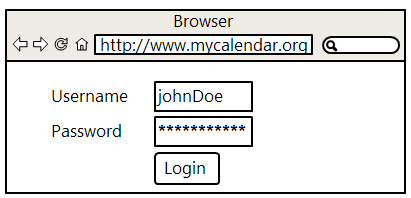
\includegraphics[width=0.8\linewidth]{Login.png}
	\caption{Wireframe model describing the Login screen.}
	\label{fig:login}
\end{figure}

\cref{fig:login} shows a wireframesketcher model of the login screen that has two text input fields and one button.
Wireframesketcher stores the models as instances of the Eclipse Ecore meta-model \cite{SBPM09} making it easy to integrate them with the Xtext-based domain-specific languages created for feature and mapping definitions.
After entering a valid ``username" and a valid ``password" the login can be executed by clicking the \textit{Login} button leading to the overview screen as shown in \Cref{fig:overview}.
The expected behavior for the Login screen is described formally within a feature definition file that contains different scenarios.

\begin{lstlisting}[captionpos=b, caption=Feature Description: Login Screen., label={lst:featureLogin}, language=dsl]
Feature Login

As a "Calendar User"
I want to "login to the calendar application"
In order to "manage my appointments"

Scenario ValidLogin
Given I am on the Login screen 
when I type "johnDoe" in the Username textfield 
and I type "Password" in the Password textfield 
and I click the Login button
then I am on the the Overview screen
and the Appointments table is visible
\end{lstlisting}

\Cref{lst:featureLogin} shows the feature description for the login screen that is divided into three main parts. 
The first part defines the feature name which in this case is \textit{Login}.
The name field is crucial for references to this file as well as for later generation and is therefore restricted to alphanumerical characters.
The second part of the feature definition contains the user story, that specifies the business value of the feature from the perspective of a certain user \cite{C.Solis.2011}.
The keyword sequences \textit{As a}, \textit{I want to}, and \textit{In order to} are predefined by the Specification Language grammar to ensure an uniform structure.
Although, the second part is optional and meaning not evaluated by the generator it is an important mechanism to document a features business value \cite{RogerioAtemdeCarvalho.2010}.
The third part describes different scenarios for each feature using grammar constructs that are a subset of the ubiquitous language gherkin \cite{wynne2012cucumber} enhanced by the functionality to reference wireframe model elements.
For a single feature there can be multiple scenarios within one file in order to describe different behavior.

The scenario in \Cref{lst:featureLogin} shows the description for a successful login.
The \textit{Login} scenario starts with the context area which sets a certain screen into focus that is thereby the starting point for the following command and assertion sections.
The first command starts with the keyword sequence \textit{When I} while all following commands in the same section begin with \textit{And I}.
The command introduced by the keyword sequence \textit{When I} is about typing the value ``\textit{johnDoe}" into the \textit{Username} textfield. 
Based on the screen in context the possible widgets, actions and their parameters are determined dynamically and proposed to the user while typing.
The \textit{When I} keyword sequences is proposed to structure the scenario description and the keyword \textit{type} is proposed dependent on the widgets on the screen in context.
The second part of the command determines on which widget the action should be executed.
At this point only such widgets are considered valid that are on the screen and applicable for the action keyword stated before.
Based on the underlying Ecore model, references can be validated at any time leading to early detection of scenarios affected by renaming or removing of widgets.
Thereby, potential errors within a test case can be determined before the test case has been executed.
The remaining two commands are concerned with entering the correct password before the \textit{Login} button is pressed.
The expected response of the application to the event triggered by clicking the button, is described in the next part of the scenario description.

The last part of the scenario description is the assertion section in which the screen content is checked after the commands have been executed.
The first assertion changes the screen context of the scenario, since it is assumed that after a successful login the \textit{Overview} screen is shown.
The following assertion statements introduced by the keyword sequence \textit{and the} are now executed in the context of the \textit{Overview} screen which means that only widgets from that screen can be referenced.

\begin{figure}[h]
	\centering
	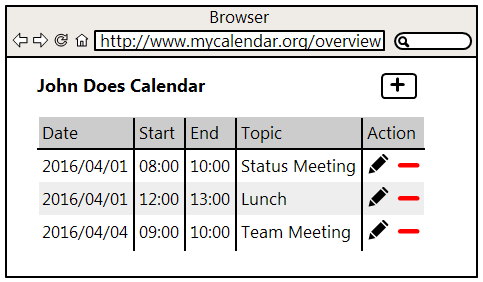
\includegraphics[width=0.8\linewidth]{Overview.png}
	\caption{Wireframe model describing the Overview screen.}
	\label{fig:overview}
\end{figure}

\Cref{fig:overview} shows the Overview screen that is shown after a successful login.
It contains a label, a table showing all known appointments and a plus button to add new entries.
To describe further scenarios for this screen a separate feature description file is created.
After having created wireframe and feature descriptions, a mapping definition depicting the wireframe elements to their implementation is required to enable the generation of automated test cases.

\begin{lstlisting}[captionpos=b, caption=Mapping Description: Login Screen., label={lst:mappinglogin}, language=dsl]
Mapping Login

locator {fragment:"#/login"}
label {"Login"}
Username{
	locator:"#username"
}
Password{
	locator:"#password"
}
Login{ 
    driver: org.sample.calendar.ButtonDriver
    locator:"#login"
}
\end{lstlisting}

\Cref{lst:mappinglogin} shows the mapping description for the Login screen.
The first part of the file states the relative URL needed to find the screen within the application which is ``\#/login". 
After the keyword \textit{label} the label of the application window, e.g. the browser window, is stated, which can be used for identifying and verifying the correct screen within the application.

The second part of the mapping files contains one entry for each widget on the screen.
As in the feature file, \textit{Username},\textit{Password}, and \textit{Login} are references to the wireframesketcher model elements.
In addition to the benefits of these references it can also be validated if all wireframe elements have been mapped.
For each widget there is one \textit{locator} which in case of a web application could be the ID of the element in the HTML document tree \cite{w3c.dom}.
For custom widgets or such that cannot be found using a simple ID mechanism a custom \textit{driver} can be specified as shown for the \textit{Login} button.
Explicitly stating a \textit{driver} will make the automated test try to find the widget using the custom \textit{driver} implementation. 
The mechanism enables the use of custom widgets without applying any changes to the screen or feature description files.

Finally, the combination of screen, feature, and mapping file is used by a generator to create a page object per screen and a test script per feature file.
The first, encapsulates all interactions, such as clicking, typing, or resolving a label, per screen in a single class.
Basis for the page objects is the combination of screen and mapping definition file.
For the example shown in \Cref{lst:featureLogin} there are two mapping definition files needed one for the \textit{Login} and one for the \textit{Overview} screen.
The second generation results are the test scripts that are generated using the information from the screen and feature files.
Every scenario is turned into a test method containing all actions and assertions.
The available default generator will create the test script in gherkin language optimized to be run with Cucumber and Selenium \cite{wynne2012cucumber}.
The page objects generated are simple groovy classes that encapsulate the interaction with the UI widgets.
Since the test scripts are based on the Cucumber framework they can be run locally, in a continuous integration environment or in a testing cloud such as SauceLab \cite{saucelab}.

\subsection{Behavior-Driven UI Testing Architecture}
\begin{figure}[h]
	\centering
	\includegraphics[width=0.8\linewidth]{SpecificationLanguageArchitecture.png}
	\caption{Behavior-Driven UI Testing Architecture.}
	\label{fig:architectureOverview}
\end{figure}

\Cref{fig:architectureOverview} shows the architecture of the Behavior-Driven UI Testing approach divided into three logical parts. 
First, the Wireframesketcher model that contains the graphical editor as well as the underlying Ecore model used to store screens and their widgets.
The functionality offered by Wireframesketcher tool has been reused completely, however, some customizations as described in \Cref{sec:WireframesketcherIntegration} were implemented.

The Specification Language is divided into two logical parts namely the feature and mapping DSL.
The wireframesketcher model is used by the feature and mapping DSL component that encapsulate the grammar definitions and the tooling implementation to support context-sensitive proposals, validations and syntax highlighting.
As shown in \Cref{fig:architectureOverview} feature and mapping DSL are completely independent from each other.
Thereby, it is possible to use Wireframesketcher and the feature DSL to concisely define requirements without taking advantage of generating any automated test cases.
Further, it is possible to only generate the page objects from the combination of Wireframesketcher model and mapping DSL while implementing the test cases manually.

As shown in \Cref{fig:architectureOverview} both generator implementations are independent and separated from the domains-specific language modules.
Thereby, generators can be switched at runtime to generate for different environments, such as web or Eclipse RCP applications, without changing the DSLs.
Both generators interact with the wireframesketcher model as well as with the respective domain-specific language definition.
The following sections will explain the modules content and their interaction in more detail.

\subsection{Wireframesketcher Integration}\label{sec:WireframesketcherIntegration} 
Wireframesketcher is a tool for creating UI descriptions for GUI based applications \cite{sanchezgui}. 
It is well integrated in the Eclipse tool-chain and offers many different UI styles, such as SWT, iOS, and HTML5  \cite{Wireframesketcher}.
The sketches are stored as instance of an Ecore model that is available in an open source repository.
To use wireframesketcher models as basis for feature and mapping descriptions the underlying Ecore model was customized.

First, the existing marker interfaces, such as \textit{ClickSupport} and \textit{SelectionSupport}, were enhanced to support more advance concepts such as \textit{DoubleClickSupport} and \textit{BooleanSelectionSupport}.
Based on the marker interfaces implemented by a widget the proposal of available actions within a scenario description are determined at runtime.
Second, the Screen class was extended to hold a \textit{name} attribute so that it can be referenced from feature and mapping definition using the Xtext default mechanisms.
Finally, the ResourceDescriptionStrategy \cite{xtext.resourcedesc} of the wireframesketcher model was extended to work with nested elements on a screen, such as widgets in containers or widgets in tables.

The adjustments described above extend the capabilities of the underlying model, but had no side-effects on the remaining wireframesketcher tooling for drawing sketches.
Consequently the model adjustments were delivered as an Eclipse feature patch that is fully inter-operable with the wireframesketcher UI functionalities so that they can be reused to create wireframe models.

In order to support more complex UIs that are composed from different application parts, wireframesketcher supports reusable components.
These components are defined as screens, however, they are marked within wireframesketcher as components and thereby become reusable for other screens \cite{Wireframesketcher.components}.
These components are very handy when for example defining a screen that is divided into different tabs.
In that case the tabbed pane is defined as reusable component and each tab is defined as one screen file.
Thereby, the common part which is the tabbed pane and all the widgets on it, e.g. shared buttons or labels, are factored out.

The additions made to wireframesketcher as well as the already existing functionalities allow users to define sound and comprehensive UI descriptions. 
Furthermore, storing the wireframe models as Ecore meta-model instances enable the integration into the Xtext based feature and mapping DSL as the following sections will illustrate.

\subsection{Feature DSL}
\subsubsection{Basic Grammar}
The feature DSL is the central part of the Specification Language defining the general structure of the document as well as the available keyword sequences.
The structure of a feature file as described in \Cref{sec:SpecifyingTheApplication} consists of three main parts.
The first part holds the feature name and an import section for the used screens and widgets.
The second part holds the user story stating the benefit of the described feature from a specific user role.
The third and most important part holds an arbitrary number of scenario descriptions for the feature file.

%TODO Is this really needed? Does not contain many interesting constructs
%TODO Add grammar for assertions
%TODO Add annotations
\begin{lstlisting}[captionpos=b, caption=Feature Grammar, label={lst:featureGrammar}, language=xtext]
Scenario:
'Scenario' name=StringOrId
GivenIamOnThe toScreenSwitch=ToScreenSwitch 
codeStatements+=CodeStatement*;

CodeStatement:
(AndI | WhenI ) AbstractCommand | 
(AndThe | ThenThe | ThenIt ) Assertion |   
ThenIAmOnThe ToScreenSwitch;

AbstractCommand:
Command|ImplementedCommand;

Command:
action=Action InThe widget=WidgetWrapper;

Action:
ClickAction |TypeAction;

ClickAction:
{ClickAction}
'click';

TypeAction:
'type' value=StringOrParam;
\end{lstlisting}

\Cref{lst:featureGrammar} shows a part of the feature Grammar that is basis for the definition of the scenario described in \Cref{lst:featureLogin}.
After setting the name, the scenario description continues with setting the context to a specific screen before the commands and assertions are defined.
As shown above an \textit{Command} consists of an actual action such as ``click" or ``type" that is followed by the widget on which it should be applied.
Actions may have parameters for example to specify what should be typed into a text field. 
In addition, there are \textit{Assertion} statements that define the third part of a scenario description containing the expected outcome of an \textit{Command}.
Within a scenario it is possible to mix both kinds of statements so that one scenario could describe a series of commands and assertions, e.g. for larger processes taking place on a single or multi screen application.   

\subsubsection{Advanced Concepts}
In addition to the capabilities shown so far the feature DSL supports advanced concepts such, external test data, composed test cases, manually implemented commands and assertion, and integration with state of the art Application Lifecycle Management tools.
 
The first advanced concept deals with integrating external test data into the feature definition by introducing ``parameters" and ``data providers".
Parameters can be used as placeholders instead of concrete text, e.g. in the \textit{BTypeAction} rule from \Cref{lst:featureGrammar}.
Within the genarated test cases the data provider is asked to replace the parameter by an actual value.
A data provider can be bound to a scenario using the Data Provider annotation that has to reference a class implementing the \textit{DataProvider} interface.
Parameters and data providers separate the feature specifications from the actual test data and thereby make them more resilient and also executable with different test data sets.

The second advanced concept introduces dependencies between scenario definitions to the grammar.
Although it is considered good practice to keep test cases independent from each other, there are situations in which a certain chain of actions is required by multiple test cases.
In the calendar application for example the tests of the edit functionality will always start with selecting an existing entry from the table of already created appointments.
Within the feature DSL this particular part of selecting an entry from the table and clicking the edit button can be factored out to an reusable scenario.
To reuse such a scenario the feature DSL offers a ``depends on" Annotation that can be added to each scenario and holds a reference to another scenario.
Based on this information the generator will generate the reusable code into the annotated scenarios test method, so that the test methods depend on each other logically, but remain independent on the source level.

Another advanced concept of the feature DSL are \textit{ImplementedCommand} statements that can be used to specify custom behavior, e.g. setting the content of a custom widget.
Within the grammar the \textit{ImplementedCommand} is a simple String, but during generation it is turned into a method within the test script that needs to be implemented manually. 
To enable regeneration of test case scripts, the custom implementation is separated from the generated code using the generation gap pattern \cite{behrens.2009}.
Besides \textit{ImplementedCommands} there are also \textit{ImplementedAssertions} that can be used within a scenario definition to define manually implemented assertions.
Although, one of the main goals of the introduced approach is to provide fully generated automatically executable test cases, there are situations in which a manual implementation is required. 
Moreover, manually implemented commands and assertions are a good basis for extending the feature and mapping grammar in order to support more advanced concepts and to replace manually implemented and maintained code in the long run.

Finally, since test cases and their results are usually managed within a test management tool, e.g. HP Quality Center or SAP Solution Manager, the feature DSL offers a connection to these systems.
In the first implementation a connector for HP Quality Center has been included that leverages the REST API of HP Quality Center.
To connect to HP Quality Center a configuration files needs to be provided holding basic information, such as URL, test project name and credentials.
In addition, every scenario can be enhanced with a Annotation stating the HP Quality Center ID of the respective test case.
Whenever a test is executed and a connection is configured the result is stored in HP Quality Center.
By integrating HP Quality Center the tests can not only be executed automatically, but are also tracked in an application lifecycle management system allowing for detailed analysis and reports.


\subsection{Mapping DSL}
One of the main advantages of the introduced approach is that it allows to generate automatically executable test cases.
The basis for this innovation is on the one hand the integration of wireframesketcher models in feature definitions and on the other hand the mapping DSL.
The latter is required to map the logical elements within a wireframesketcher model such as \textit{Screen} or \textit{Widget} to their implementation.
As shown in \Cref{lst:mappinglogin} mapping files are defined per \textit{Screen} and consist of two parts.

\begin{lstlisting}[captionpos=b, caption=Mapping Grammar, label={lst:mappingGrammar}, language=xtext]
BUrl:
'locator' '{'
	('fragment' |'path') ':' mPath=MExpression
	'}'
;
\end{lstlisting}

The first holds the name of the mapped screen and an ``locator" attribute containing a relative URL to find the screen within the application.
In the example used above the ``locator" attribute holds a fragment of an URL, however as \Cref{lst:mappingGrammar} shows it is also possible to introduce the ``MExpression" by the keyword ``path" to define a menu path.
The later is often used in SWT application, since their views are usually accessible via a menu.  
In addition, a ``label" attribute can be specified to verify that for example in an web application the name of the browser window matches the label.
The second contains the mapping information for all widgets on the particular \textit{Screen}.
The widget mappings consists of a reference to the wireframesketcher model element, the ``locator" attribute, and an optional ``driver" attribute.
The locator attribute is a String value that exactly identifies the widget within the screen.
For a web application this might be the ID of an element in the DOM tree.
The optional driver attribute holds a String value that represents a class on the classpath of the test project that is used interact with the widget.
Specifying a custom driver allows to use custom widgets and their custom functions, e.g. to identify them.

Since their is deep knowledge about the implementation necessary to fill out the mapping file, it should be created and maintained by the responsible developer. 
Because developer resources are usually very limited especially when it comes to writing tests, the introduced approach tries to reduce developer involvement.
First, this is achieved by having one mapping file per Screen that is separated from the actual test script, so that the mapping definition is structured in known chunks (Screens in this case). 
Second, the references to the EClasses representing the wireframesketcher widgets allows for extended validation support, e.g. automatically checking if all widgets of a screen are mapped.
Finally, the reusable component feature of wireframesketcher is supported by the mapping DSL, so that reusable screens only have to be mapped once.

\subsection{Generator}\label{sec:Generator} 
After having defined wireframesketcher, feature and mapping descriptions a generator turns all instances the three artifact types into automatically executable test specifications.
As shown by \Cref{fig:architectureOverview} there are two kinds of generators that are loosely coupled to the DSLs and the wireframesketcher model.
The default implementation is a generator for web applications, that generates Cucumber specification files.
In addition, there has been a proprietary generator for a SWT based RCP application.
Since the feature and mapping files are created within Eclipse projects the generator to use can be defined per project.
Within the properties of an Eclipse project any generator that is registered through the Eclipse Extension mechanism can be selected.
Before a generation starts, the application asks the Property Service which generator should be executed and then tries to find that generator within the registered extensions.
Being able to change the generator at any time makes the whole approach very flexible, however, it also adds restrictions to the DSLs.
To allow changing generators lately the DSLs need to be generic to a level that different UI frameworks and concepts such as web, SWT or Swing based applications can be described.
In addition, the DSLs should support the requirements engineer during the creation of test specifications by giving reasonable proposals.

In order to interact with the widget on a screen, the mapping generator create an Page Object \cite{fowler.2013} per Screen file.
Within these page objects all interaction with the screen and its widgets are encapsulated.

\begin{lstlisting}[captionpos=b, caption=Generated Page Object, label={lst:MappingGenerated}, language=dsl]
class LoginScreen {
	static url = "#/login"
	static at = { waitFor { title == "Login" } }
	
	static content = {
		username (required: true) { module org.boomslang.module.BoomslangModule, $("#username") }
		password (required: true) { module org.boomslang.module.BoomslangModule, $("#password") }
		submit (required: true , wait:true) { module org.sample.calendar.ButtonDriver, $("#login") }
	}
}
\end{lstlisting}

\Cref{lst:MappingGenerated} shows the page object for the Login example that is generated as groovy file.
The page object is in Groovy programming language because it interacts well with the Cucumber test specification that is generated by the feature generator.
The structure of the generated page object is very close to the mapping file because in the end the mapping DSL is just an slightly enhanced page object description.
The main part of the screen is the ``content" attribute that holds the locators for all the widgets on the screen.
If a ``driver" is specified in the mapping file, it is referenced here and during runtime of the test cases the Cucumber framework tries to find the class on the classpath.

\begin{lstlisting}[captionpos=b, caption=Generated Feature File, label={lst:featureGenerated}, language=dsl]
	def "ValidLogin"() {
	given:
	to (org.specification.calendar.LoginScreen);
	
	when:
	username.value $username
	and:
	password.value $password
	
	then:
	at OverviewScreen
	and:
	waitFor { appointments }
	
	where:
	$password | $username
	"Password" | "johnDoe"
}
\end{lstlisting}

Although the feature Generator is logically separated from the mapping generator it relies on the page objects.
Within the generated Cucumber specification the page objects are instantiated and used to interact with the application.
\Cref{lst:featureGenerated} presents the generated cucumber test script for the Login example. 
Like the page objects the test script's structure is very close to the structure of the feature file it is generated from.
This is due to the fact that the feature DSL itself introduces no new concepts to the general structure of a feature or scenario description.
The innovation lies in the connection to the page object that is fully generated and therefore makes the test scripts ready to be executed without any further manual adjustments.

One though enhancement compared to the feature file is in the ``where" section that holds the data used in the test scenario.
This section is a feature of the underlying Cucumber framework that enable the test to run with different data input. 
The test case will be executed for each line of data, so that this way of generating makes it easy to run the same script multiple times with different test data.

Since the test cases can be executed without further manual interaction the generator can be included in a continuous integration environment.
Whenever the application under test is builded the test generator is called to turn Wireframe, feature and mapping files into test specifications before these are executed during a the build.
%TODO Source? BDD Characteristics?
By integrating the generator into the development process the basic principle of test driven development which is: fail, refactor, pass can be ensured.

%TODO Do I want to mention keyword-driven testing?
%Since a subset of the BDD ubiquitous language is used for test case definition the approach falls into the category of keyword-driven UI tests.
%TODO Quelle Keyword driven tests und die vorteile
%Besides the advantages of keyword driven testing as described by [..], the Specification Language as central part of the approach introduces additional benefits.
%First, reusing well-known constructs from BDDs ubiquitous language lowers the barrier for new users.
%Further, the ubiquitous language has been tested and adjusted to project needs so that it has become a very concise for defining behavior and scenarios.

%TODO Components
\section{Discussion}\label{sec:Discussion}
%Wrap up
%General Use Cases
The approach presented in this paper focuses on generating automatically executable test cases from scenario descriptions in the format of the behavior-driven developments ubiquitous language.
%TODO Quelle Testing pyramid
Looking at the testing pyramid as defined by [..] the Behavior-Driven UI test cases are from the top level area.
Consequently, the scenario descriptions should focus on testing different UI behavior e.g. forcing error dialogs and page flows.
Further, the test cases can cover very basic UI behavior like sorting and filtering of tables or opening all menus and tabs of the application. 
Although, the Specification-Language allows for dynamically provided test data, it is not meant to build data intensive test cases that are more likely to be defined on the service test layer.

%Integration into the development process
The Behavior-driven UI testing approach aims to integrate well with existing development processes. 
Therefore, the presented approach is not introducing new tools or techniques, but on the contrary is combining artifacts from different areas to leverage potential benefits.
First, the Wireframesketcher tool is used to define wireframe models ranging from simple one page application to complex multi-component perspectives.
Second, the feature-DSL enhances the industry proven and widely accepted concepts from the ubiquitous language with references to widgets from the wireframe models.
Third, the Mapping-DSL enables for fully generated test cases and in addition minimizes the involvement of critical developer resources. 
Finally, the plugable generator architecture comes with a standard implementation that can be used for web-application that can be replaced to target company- or company-specific frameworks.
In addition, the textual feature descriptions are edited and managed together with the source code of the application.
Thereby, during every build test cases are executed and on top of that the results are stored in professional test management tools such as HP Quality Center.

%First experience

First experiences were gained in context of the development of a banking application. 
The developed software consist of four components, one has a javascript frontend and the other three are based on the Eclipse SWT UI framework.
The wireframe models were instances of the same meta-model so that they both could be integrated with feature and mapping DSL, although, the graphical representation was slightly different.
In addition to using the same wireframesketcher meta-model it was proven possible to use the same feature and mapping DSL to describe the behavior and widget mapping.
The only, exception is the ``locator" attribute within the mapping file that contains two different keywords for introducing either a URL expression or a menu path to be followed.

Within the projects that used the Specification Language wireframesketcher was already known as well as JBehave for defining feature descriptions.
As a consequences the Specification Languages could be used by business analysts and developers after only 2 hours training.
Furthermore, in comparison to manually writing automated test cases the time a developer spent decreased significantly by limiting their efforts to providing the mapping definitions.
However, since there were only four projects involved additional research is required.
The feedback from business analysts was specially emphasizing the advanced validation possibilities that helped to keep wireframes and requirements specifications congruent.
In addition, the concept of reusable components as introduced by wireframsketcher that is supported throughout the whole Behavior-driven UI testing approach was appreciated by business analysts to create concise scenario descriptions.
 
In contrast to the idea of fully generating all test cases the practical experience has shown that there are cases in which a flexible way to include manually implemented code is necessary. 
The implementation commands and assertions support this need and also give hints for concepts that should be supported by future versions of the Specification-Language.


\section{Conclusion}\label{sec:Conclusion} %and Future Work
The specification Language introduced by this paper combines the ubiquitous language from the behavior-driven design approach with wireframesketches to generate automatically executable test cases.
The implementation presented supports basic widgets such as text fields, buttons, and tables, however, there are more standard widgets such as tabbed panes or calendar chooser that should be supported by future versions.
Besides being able to handle custom widgets using implemented commands, and assertions, and custom drivers, it is to be discovered which widgets are to be supported by the default implementation.
With the flexible architecture of the introduced approach it is possible to support all kinds of custom widgets from wireframe through feature and mapping file up to the generator.

Especially, the use of the ubiquitous language makes the language to learn for people already familiar with BDD. 
In addition, every feature descriptions reads like a grammatically correct sentence so that they can even be used for describing the behaviour of the application without leveraging the benefits of automatically generated test cases.
By combining existing artifacts from different areas of the software development process the Behavior-Driven UI testing approach leverages the full potential of these artifacts.
At the same time Designer, Business Analysts and Developer remain in their known environment, but work together on a more formal level. 

All in all, the Behavior-Driven UI testing approach enhances the widely accepted Behavior-Driven development process leading to a more sophisticated tooling to specify and maintain automatically executable test cases.
The integration of wireframesketcher models, Specification-Language and generators was tested successfully in four projects from the banking sector. 



%Future work:
%Include more widgets and container types
%How to integrate test cases
%Expand the concept to Service Testing --> Enable architects to specify service tests with a BDD language. 
%In many projects requirements engineers or architects are heavily involved in the task of defining services and their input output parameters.
%However, the description is often only a textual description of the input and output parameter and potential exceptions. 

%TODO More commands and actions like table, trees and lists that can be elaborated in more detail 

%TODO Future work: How to compose tests scripts for UI comming from different components? First expecting every component to deliver a tested UI, but who is repsonsible for integrated tests and where should they be managed?

%TODO Bring UI desription and behavior description closer together leading to an more sophisticated BDD tooling

%\newpage
%
% The following two commands are all you need in the
% initial runs of your .tex file to
% produce the bibliography for the citations in your paper.
%IMPORTANT directly embedded
\bibliographystyle{abbrv}
\bibliography{specification_driven_testing}  % sigproc.bib is the name of the Bibliography in this case

%\begin{thebibliography}{10}
%\end{thebibliography}

% You must have a proper ".bib" file
%  and remember to run:
% latex bibtex latex latex
% to resolve all references
%
% the ACM needs 'a single self-contained file'!
%
%\balancecolumns
\begin{comment}
\appendix
%Appendix A
\section{Headings in Appendices}
\subsection{References}
Generated by bibtex from your ~.bib file.  Run latex,
then bibtex, then latex twice (to resolve references)
to create the ~.bbl file.  Insert that ~.bbl file into
the .tex source file and comment out
the command \texttt{{\char'134}thebibliography}.
%\balancecolumns
\end{comment}
\end{document}
